\documentclass[11pt,a4paper]{article}
\usepackage{fontspec}
\setmainfont{TeX Gyre Pagella}
\newfontfamily\headfont{Inter}[UprightFont=*-ExtraBold,BoldFont=*-ExtraBold,Extension=.otf,Path=/usr/share/fonts/opentype/inter/]
\usepackage[a4paper,margin=2.3cm]{geometry}
\usepackage{graphicx,booktabs,float,caption,array,xcolor,longtable}
\usepackage{xurl}
\usepackage[hidelinks]{hyperref}
\usepackage{titlesec}
\usepackage[round]{natbib}
\usepackage{setspace}
\setstretch{1.05}
\renewcommand{\topfraction}{0.9}
\renewcommand{\bottomfraction}{0.8}
\renewcommand{\textfraction}{0.1}
\renewcommand{\floatpagefraction}{0.75}
\setlength{\parindent}{0pt}
\setlength{\parskip}{0.55em}
\titleformat{\section}{\headfont\Large}{\thesection}{0.8em}{}
\titleformat{\subsection}{\headfont\large}{\thesubsection}{0.8em}{}
\captionsetup{font=small,labelfont=bf}
\urlstyle{same}
\hypersetup{pdftitle={The Gough Map: Britain's Oldest Road Map, Measured},pdfauthor={Tristan Hotham}}

\begin{document}
\begin{center}
{\Large\bfseries The Gough Map: Britain's Oldest Road Map, Measured\par}
\vspace{0.4em}
{\large Shape and distance on a map of about 1360:\\157 way stations located on the parchment and 169 written mileages checked against the roads\par}
\vspace{1.2em}
{\large Tristan Hotham\par}
\vspace{0.3em}
{\small Independent researcher\\
ORCID: 0000-0003-4931-9349\\
DOI: https://doi.org/10.5281/zenodo.24043678\par}
\vspace{0.8em}
2026
\end{center}

\begin{quote}
\small
\begin{center}\textbf{Abstract}\end{center}
The Gough Map (Bodleian Library, MS. Gough Gen. Top. 16), drawn about 1360 with east at the top, is the oldest surviving map of Britain to show a road network: red lines join way stations and most carry a distance in Roman numerals. I combine the GIS database of Oksanen and Brookes, which gives the true positions of its 179 way stations, its 188 red lines with their figures and the real routes they most likely stand for, with the positions of 157 way stations (88\%) located by eye on a high-resolution photograph of the map. A similarity fit turns the map 95\textdegree{} from north-up; at its average scale the median way station is misplaced by 17.6 km, and an affine fit adds little (stretch 1.11). Wales is drawn at 1.22 times the average scale with a median error of 33.2 km; Scotland, checked with a few control points, is compressed. One written mile corresponds to a median 2.08 km of road (1.29 statute miles) and 1.89 km in a straight line; 72\% of 169 figures are within 25\% of the road length at that rate. The written figures are more accurate than the drawn lengths of the same lines (median error 13\% against 31\%), and summed along the network they give London to York as 420 km against 424 km of road. Of the 4,505 km of road under the red lines, 35.4\% is Roman; the figures are equally good on Roman and later roads.

\textbf{Keywords:} Gough Map; medieval cartography; road networks; itineraries; map distortion; historical GIS
\end{quote}

\section{Introduction}
The Gough Map is a map of Great Britain on two pieces of parchment, about 115 by 56 cm, in the Bodleian Library, Oxford. It is named after the antiquary Richard Gough, who acquired it in 1774, and is usually dated to about 1360, with later revisions \citep{parsons,delano}. It is oriented with east at the top. Its most celebrated feature is a network of thin red lines joining towns, most of them with a distance written beside them in Roman numerals: the earliest surviving road map of Britain \citep{lilley,delano}. How the network was compiled, and how it relates to real roads, has long been debated; \citet{ads} recently published a GIS database that identifies, for each red line, the most likely real route on the ground, and dates its parts from Roman roads to the road books of the seventeenth and eighteenth centuries.

This paper uses that database to ask two questions that need both the map and the ground: how wrong is the map's shape, region by region, and how right are its written distances? The first requires the positions of the way stations on the map itself, which the database does not give; I located them by eye. The study accompanies an interactive comparison of the map and an ink map of the same roads (\url{https://maps.tristanhotham.com/gough-map/}).

\section{Data}
\textbf{The road database.} \citet{ads}: 179 way stations (settlements joined by a red line) in British National Grid, with modern name, historic county and legibility of the name on the map; 188 red lines between them with the written figure (19 absent or faded); and 455 route segments, about 4,542 km in all, each with a period code, a category (Roman road, a road on Cary's maps, modern road), Margary numbers for Roman roads \citep{margary}, and the evidence used. The period codes are numeric and I could not reach the published key; from the categories and comments I read them as: 1 Roman road; 2 evidence before Domesday (1086), such as Anglo-Saxon charter bounds; 3 dated medieval evidence after Domesday, mostly bridges; 4 other medieval evidence, such as the routes of Gerald of Wales or the 1334 lay subsidy; 5 known only from the early modern road books \citep{ogilby}; 6 river; 0 undated or modern road. Results by period depend on that reading.

\textbf{The map.} A photograph of the whole map, 12,224 by 6,021 pixels, from Wikimedia Commons (\url{https://commons.wikimedia.org/wiki/File:Gough_Kaart_(hoge_resolutie).jpg}), a faithful reproduction of a public domain work. \textbf{Outlines.} Natural Earth \citep{ne}.

\section{Methods}
\subsection{Locating the way stations}
No published table gives where each way station is drawn. I located them on the photograph at full resolution, on gridded crops. I started from unmistakable towns (London, York, Exeter, St David's), fitted an affine and then a thin-plate spline from the National Grid to the image, and used it to predict where each remaining town should be drawn. Each was then identified on the crop: by its label where legible (33, ``high''), by the right town drawing at the end of the right red line with the right numeral (56, ``medium''), or with real doubt, usually among faded drawings or several candidates (68, ``low''). 22 could not be placed, 6 of them in Cornwall, where the parchment is worn. Because the map has no red lines in Scotland, I added 6 control points read the same way: Orkney, the Isle of May, the Bass Rock, Perth and the two ends of Hadrian's Wall (Table~\ref{tab:located}). As a consistency check, a smooth fit through all other points predicts each point to within a median 8.1 km.

\subsection{Shape}
Positions in National Grid kilometres were fitted to image pixels (with the image $y$ axis turned up) by least squares, first with a similarity (one scale, one rotation, a shift), then with a general affine transformation \citep{tobler}. A way station's misplacement is the distance between its true position and its map position taken back to the ground through the inverse of the overall similarity: how far the map puts it from where a correctly shaped map at the same scale and orientation would. Each region of at least six located places (groups of historic counties) has its own similarity fit, reported as its scale relative to the whole map and its rotation relative to the map's mean rotation, and an affine fit whose ratio of singular values measures stretch. For the figures, a thin-plate spline \citep{bookstein} with light smoothing carries the National Grid and the modern coastline onto the image, and back again at the overall similarity (the ``Gough shape'' of England and Wales). The spline is unconstrained far from located points and is not used for Scotland.

\subsection{Distances}
The route segments were joined into a network at the vertex level (vertices within 30 m merged; loose ends joined to the nearest vertex of another segment within 400 m). Each way station was put on the nearest vertex (median offset under 0.1 km, at most 1.7 km, added to the length), and each red line's road distance is the shortest path between its two way stations over segment lengths as given in the database. Straight-line distances are in the National Grid. For each of the 169 red lines with a legible figure, kilometres per written mile is road (or straight) distance divided by the figure; a figure ``agrees within 25\%'' when the figure times the median rate is within a factor of 1.25 of the road distance. The drawn length of a red line is the image distance between its two located stations divided by the overall similarity scale. Journeys are shortest paths over the red lines weighted by the written figure, with faded figures filled from the road length at the median rate.

\section{Results}
\subsection{The two maps}
Figure~\ref{fig:maps} shows the located way stations on the photograph with the 25 km National Grid bent to fit. The grid is remarkably regular over England, tightening towards the north and opening out over Wales.

\begin{figure}[tbp]\centering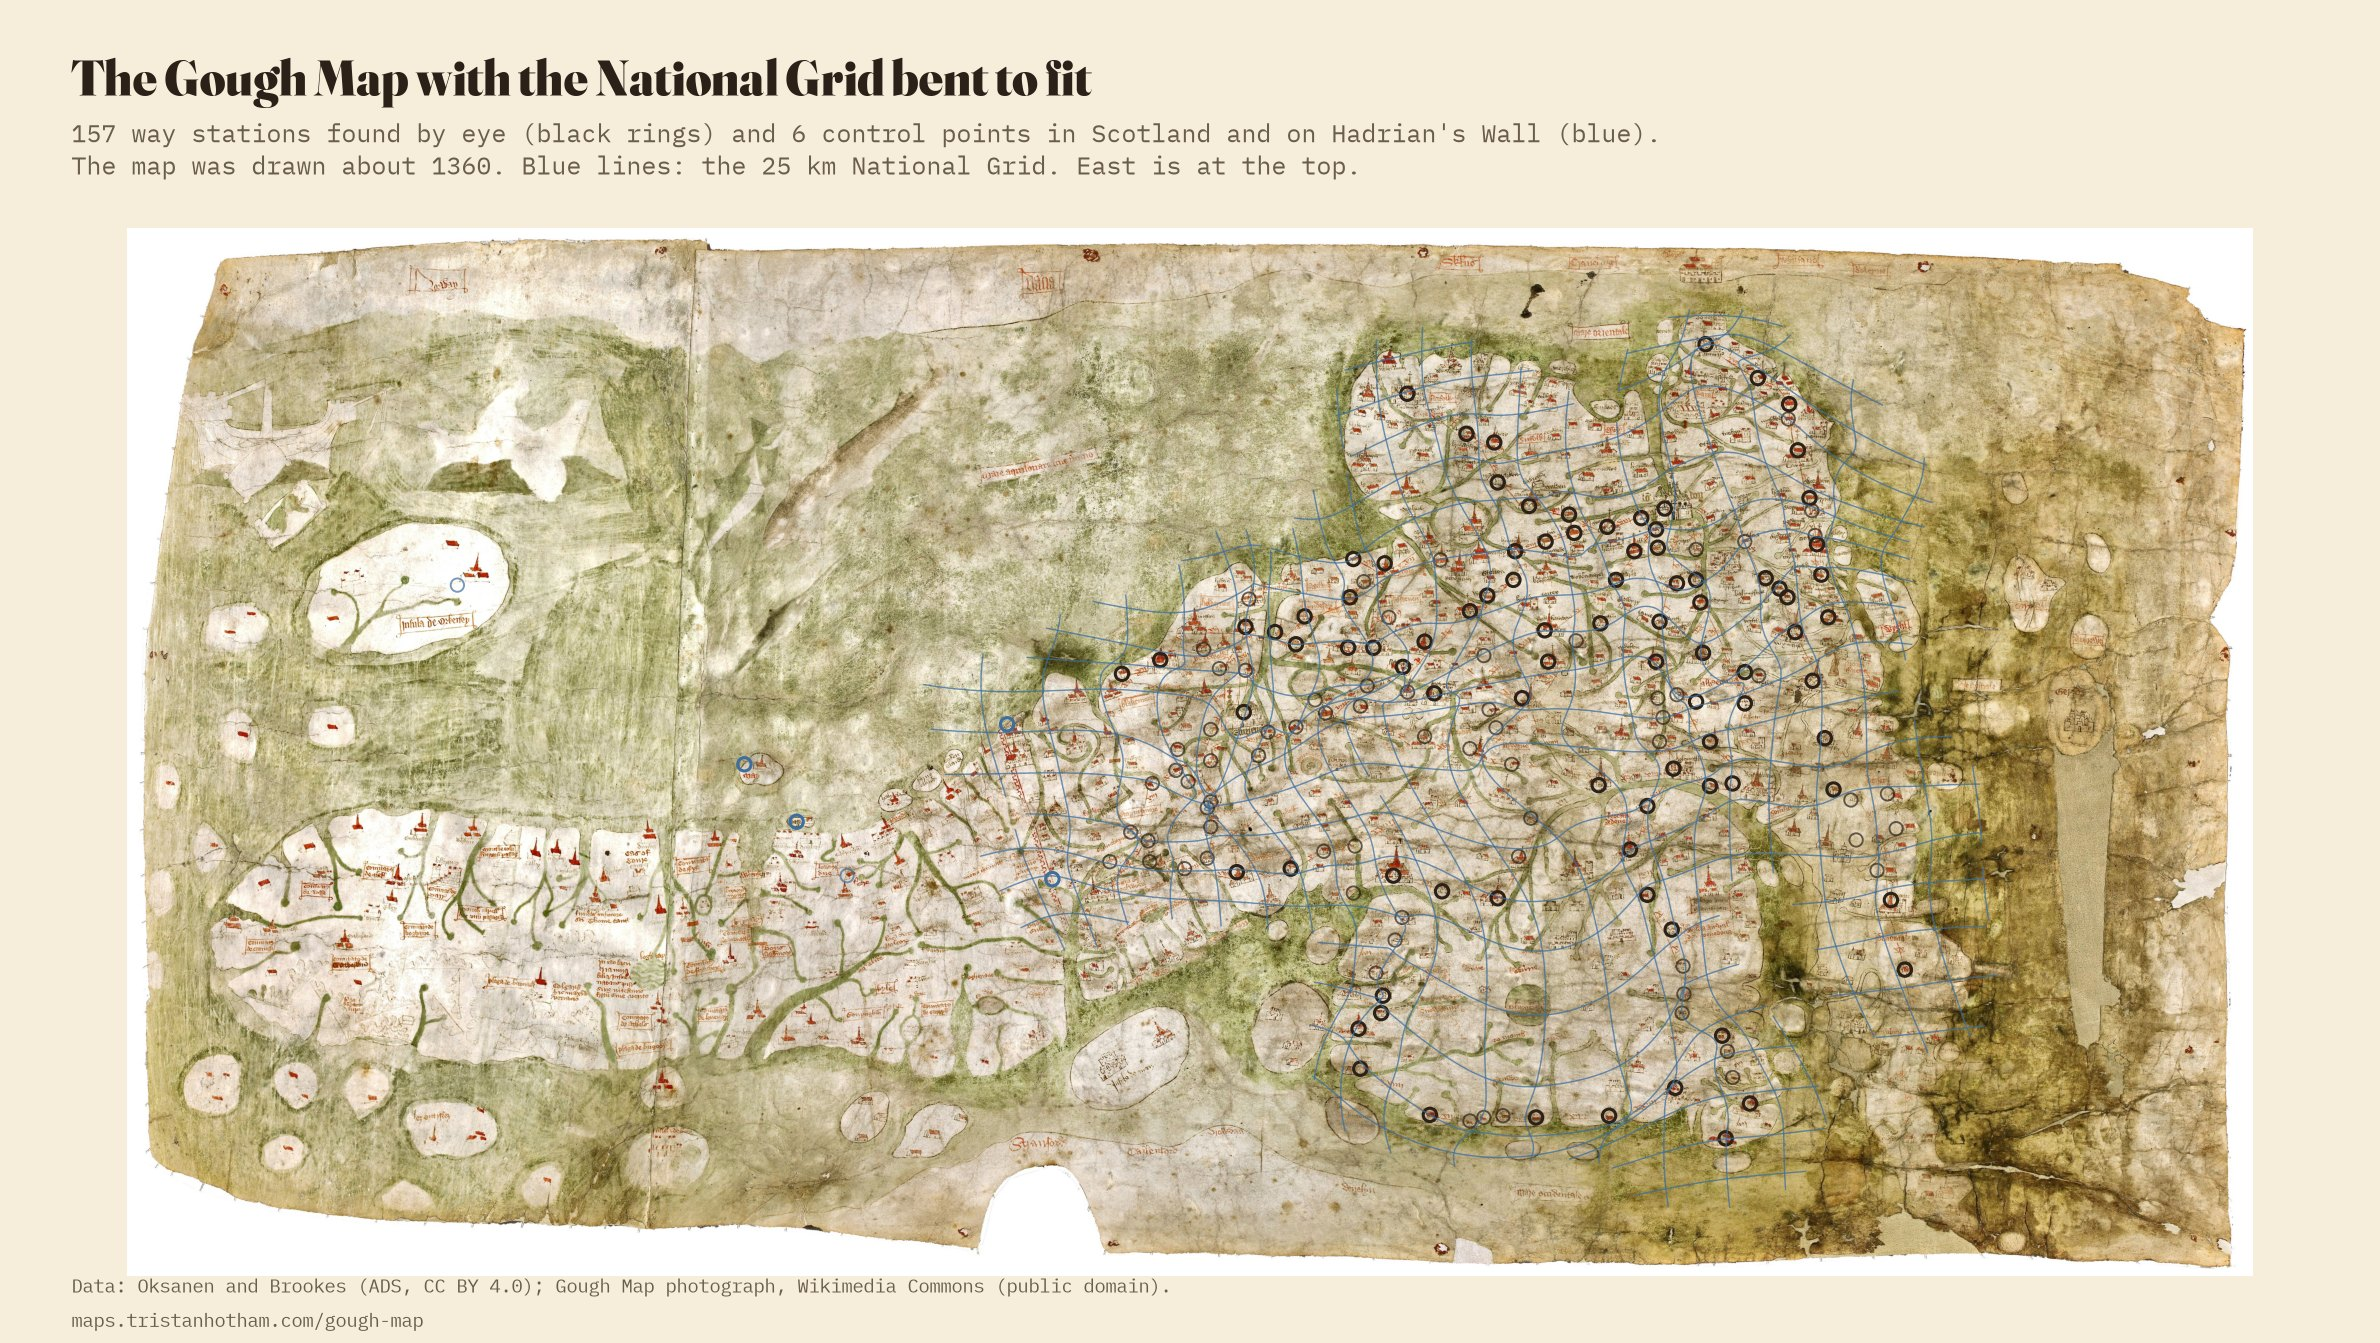
\includegraphics[width=\textwidth]{f_maps.jpg}
\caption{The Gough Map with the way stations located (black rings), the control points (blue) and the National Grid at 25 km carried onto the image by a thin-plate spline. East is at the top.}\label{fig:maps}\end{figure}

\subsection{Shape}
The similarity fit turns the map 95\textdegree{} anticlockwise from north-up (96\textdegree{} with high and medium confidence points only): east at the top, with a further lean of about 4.6\textdegree. At the overall scale, the median way station is misplaced by 17.6 km and 76\% are within 25 km; the root mean square error is 31.3 km. An affine fit barely improves on this (stretch 1.11; 1.07 for the surer points), so the map has no strong overall squeeze in one direction. Errors vary by region (Figure~\ref{fig:arrows}, Table~\ref{tab:regions}). The north of England (12.6 km) and the south-east (13.9 km) are best; the Midlands, East and South-west lie near 20 km. Wales is drawn at 1.22 times the overall scale and its way stations are misplaced by a median 33.2 km; the five worst-placed way stations are all on the coast of Cardigan Bay, led by Aberystwyth (70 km). The north of England is drawn small (0.90).

\begin{figure}[tbp]\centering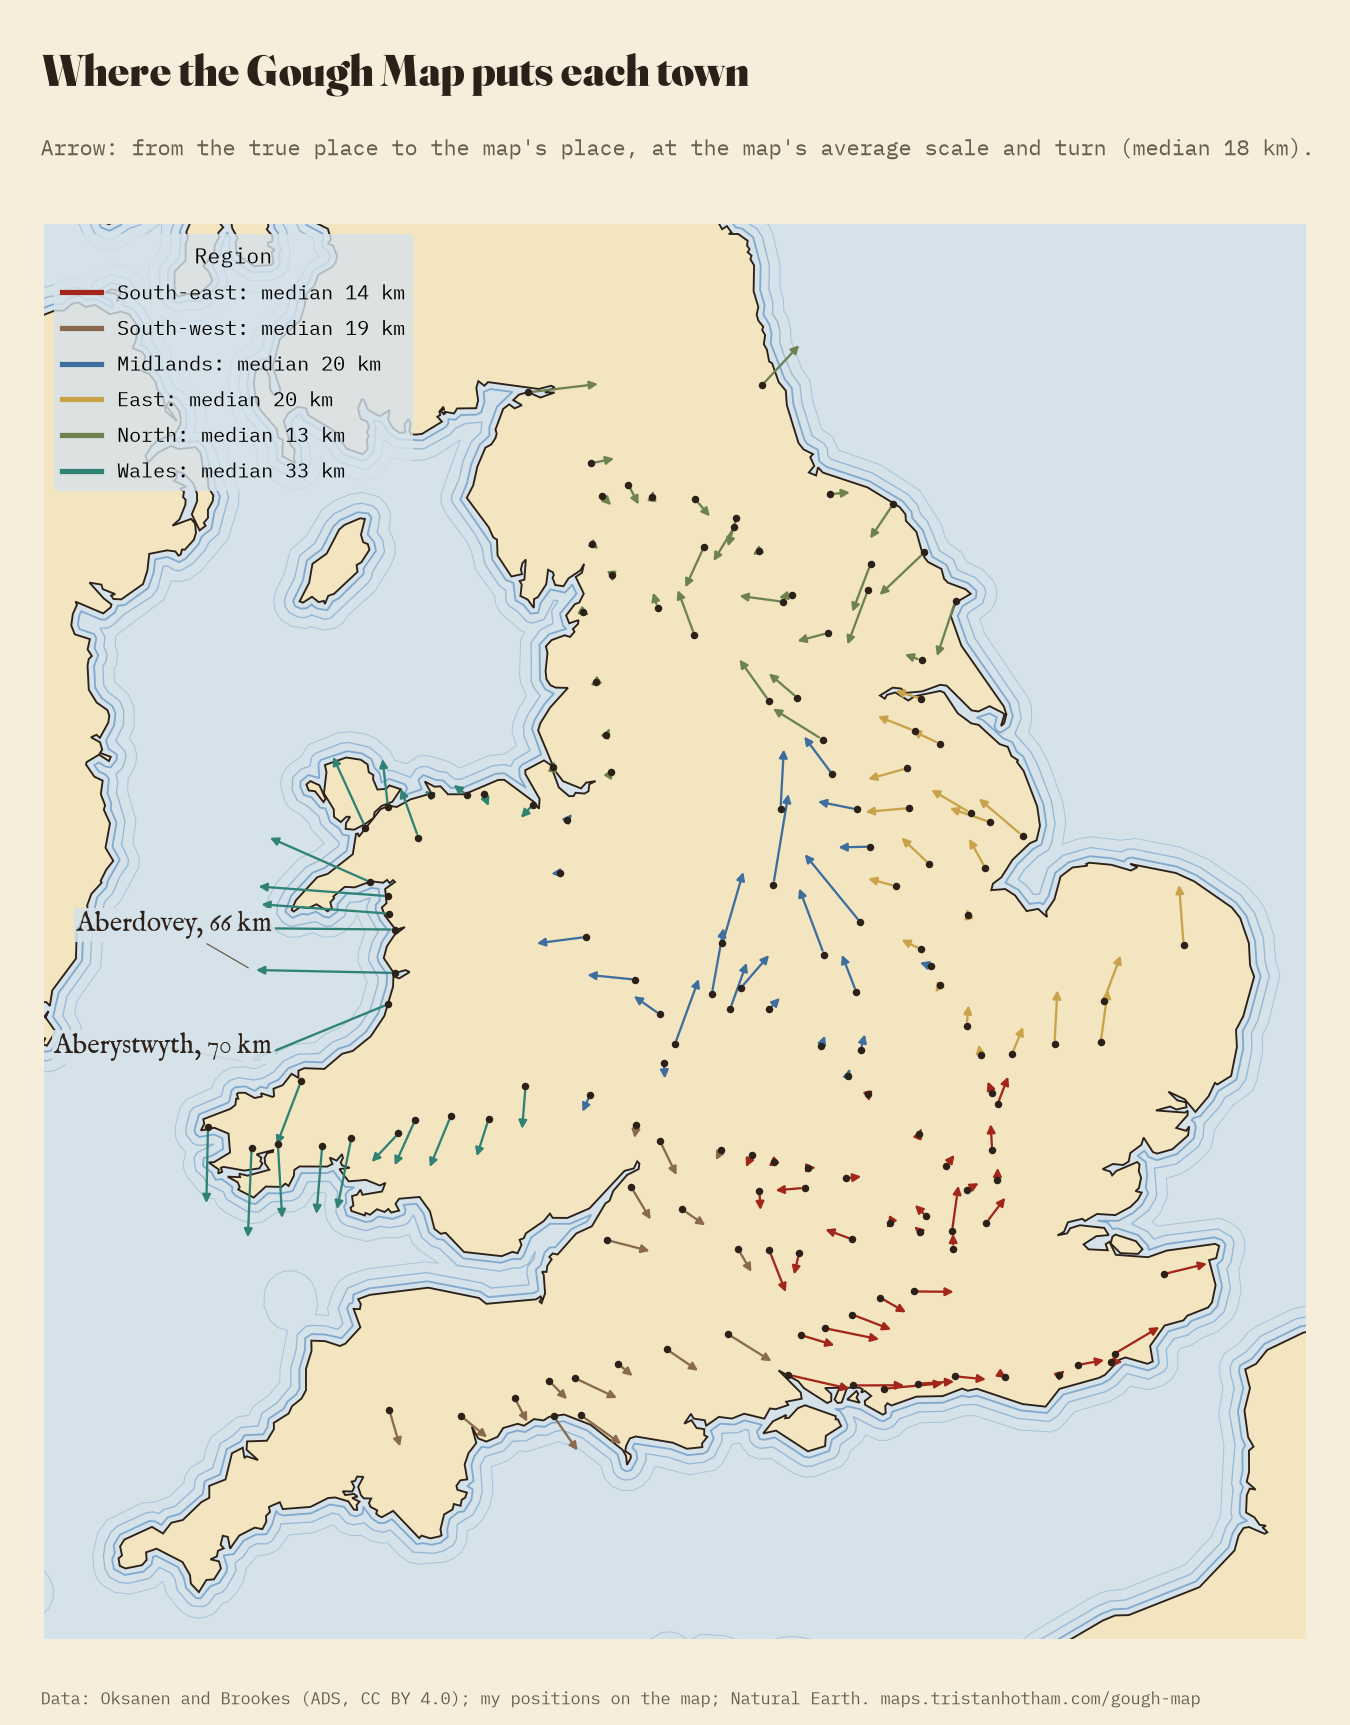
\includegraphics[width=.82\textwidth]{f_arrows.png}
\caption{Misplacement of each located place: arrow from the true position to the map position at the overall scale and rotation, coloured by region.}\label{fig:arrows}\end{figure}

\begin{table}[tbp]\centering\small\caption{Regions (groups of historic counties): located places; median misplacement at the overall similarity (km); RMS residual of the region's own similarity fit (km); its scale relative to the whole map; its rotation relative to the whole map (degrees, anticlockwise positive); and the stretch of its affine fit.}\label{tab:regions}\begin{tabular}{lrrrrrr}\toprule Region & Places & Misplaced & RMS & Scale & Turn & Stretch\\\midrule
South-east & 39 & 13.9 & 10.3 & 1.04 & +7.6 & 1.09\\
South-west & 17 & 19.1 & 7.4 & 1.01 & +3.0 & 1.11\\
Midlands & 25 & 20.3 & 17.8 & 1.02 & +4.9 & 1.07\\
East & 21 & 19.6 & 7.4 & 1.01 & +10.7 & 1.13\\
North & 33 & 12.6 & 15.7 & 0.90 & -6.7 & 1.10\\
Wales & 24 & 33.2 & 22.4 & 1.22 & +5.2 & 1.23\\
\bottomrule\end{tabular}\end{table}

North of the Wall the map is much less reliable. The Wall's ends are within about 31 km of their places. Orkney is 450 km from the middle of the Wall but drawn at 356 km (0.79), and is misplaced by 246 km; Perth is drawn at 0.67 of its distance, while the Isle of May and the Bass Rock, at the mouth of the Forth, are pushed out (1.24 and 1.10). With four points these are indications only. Figure~\ref{fig:morph} shows England and Wales in the map's shape.

\begin{figure}[tbp]\centering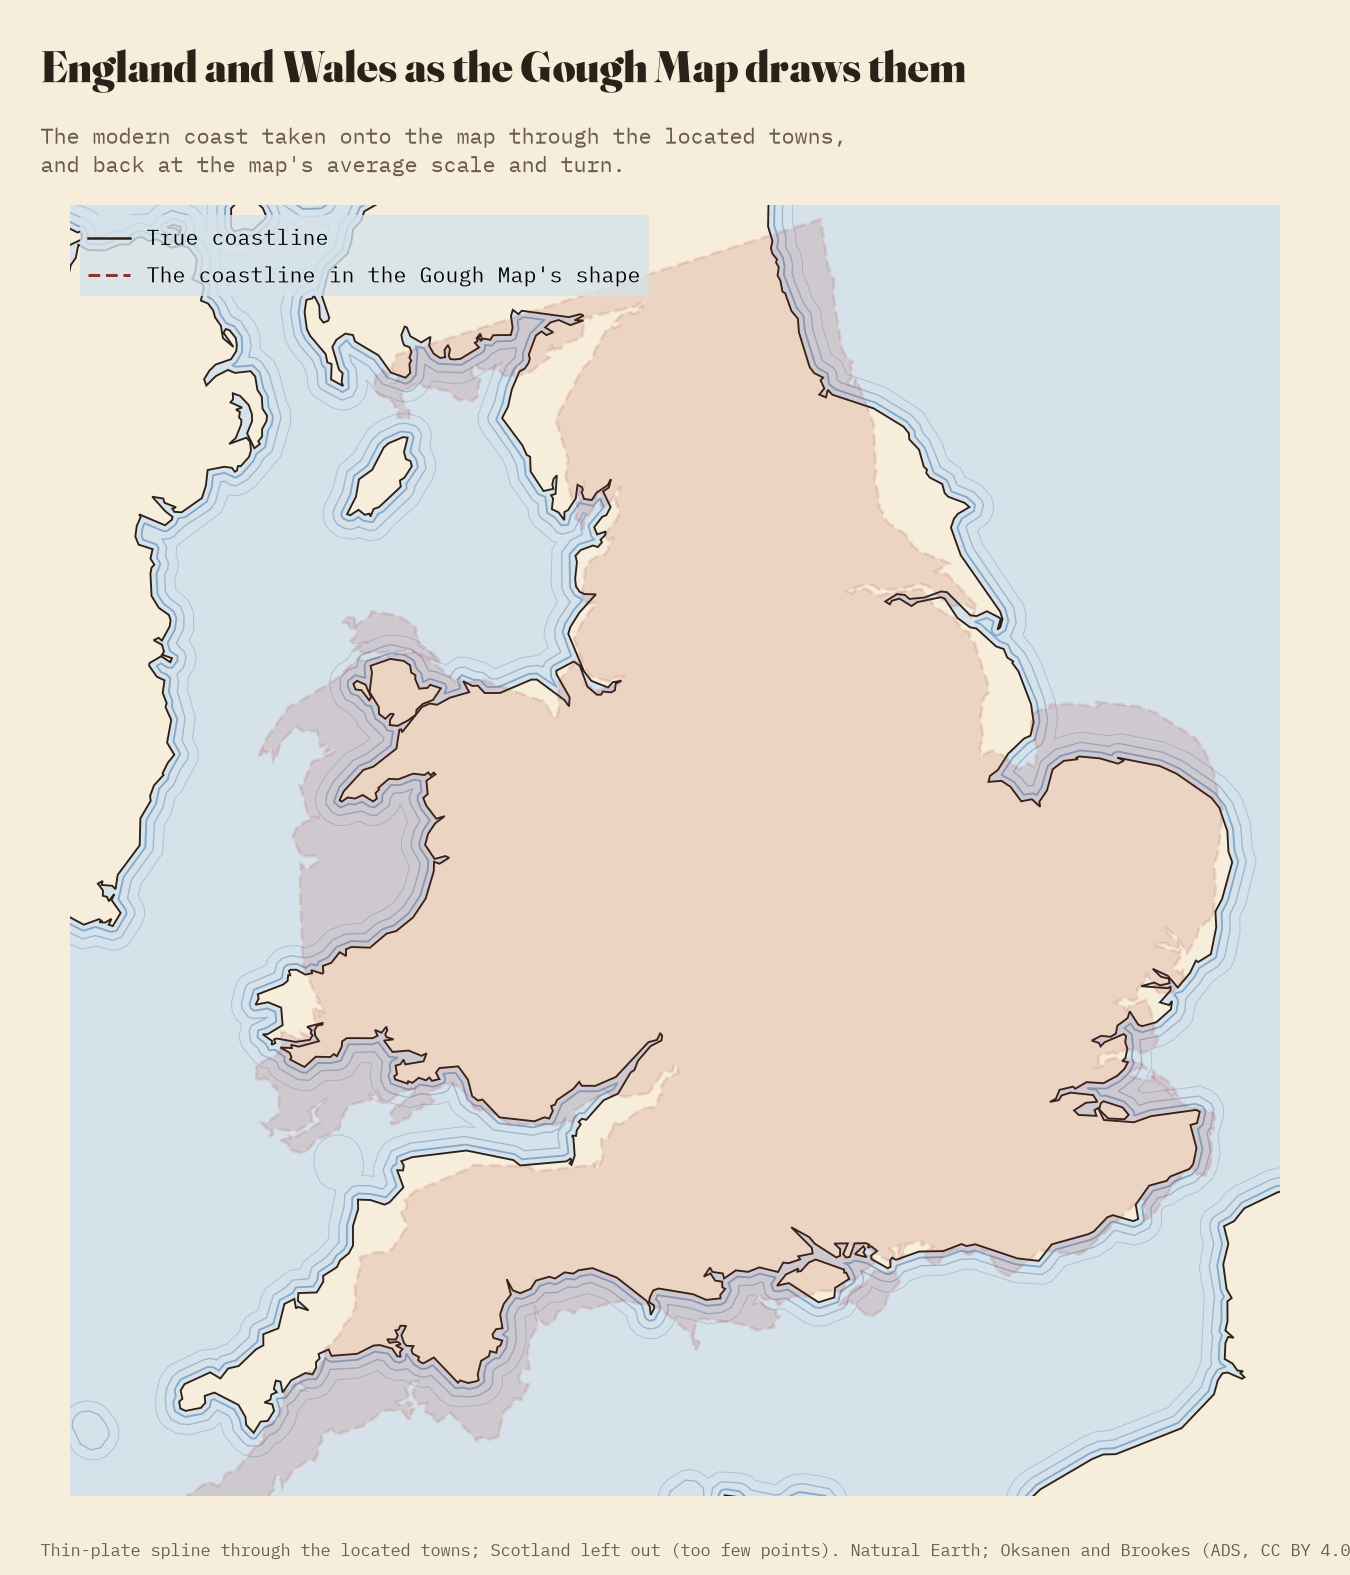
\includegraphics[width=.8\textwidth]{f_morph.png}
\caption{The modern coastline of England and Wales carried onto the map by the thin-plate spline and back to the ground at the overall similarity: the island as the Gough Map draws it.}\label{fig:morph}\end{figure}

\subsection{The written miles}
One written mile corresponds to a median 2.08 km of road (interquartile range 1.85 to 2.37) and 1.89 km in a straight line, or 1.29 and 1.17 statute miles; the roads are a median 1.10 times the straight line. At 2.08 km a mile, 72\% of the 169 figures agree with the road within 25\% and 89\% within 50\%; the rank correlation between figure and road length is 0.74 (Figure~\ref{fig:miles}). The rate is lower for long lines (1.93 km for figures above 12) than for short ones (2.21 km for 8 or less), and ranges by region from 1.86 (South-west) to 2.34 (Midlands). The largest misfits (Rye to Winchelsea, 8 miles for 4.7 km; Barmouth to Llanenddwyn, 12 for 7.7) look like copying errors or misattributed figures.

\begin{figure}[tbp]\centering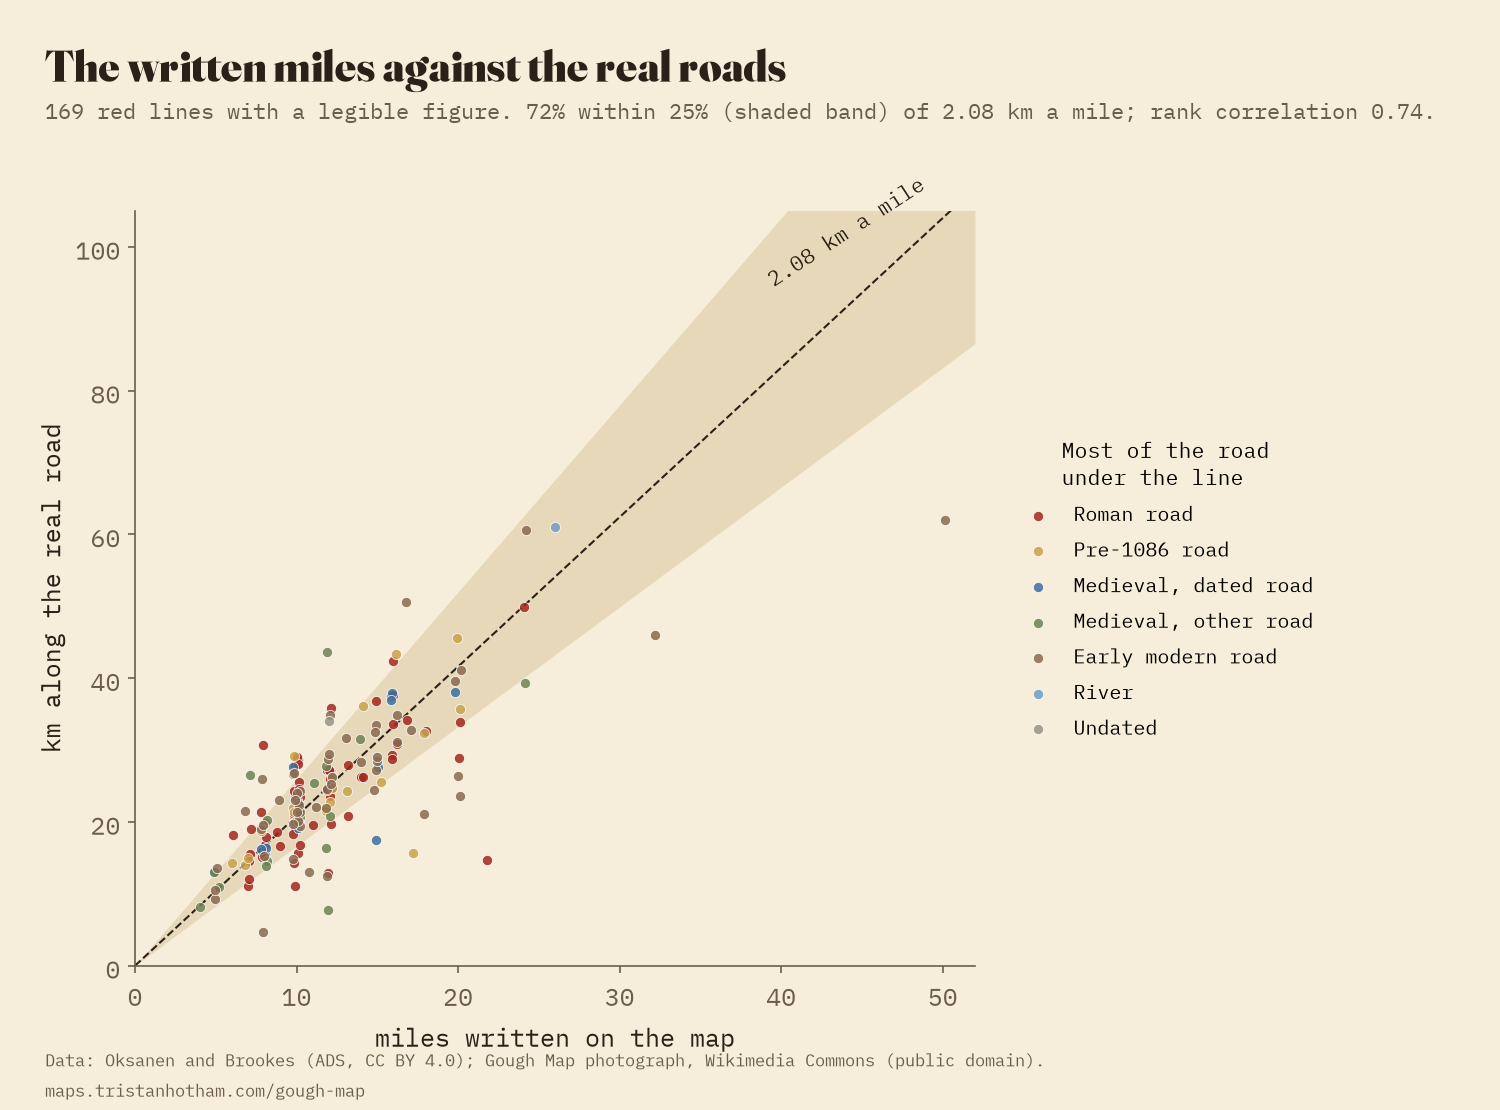
\includegraphics[width=.9\textwidth]{f_miles.png}
\caption{Written figure against road length for each red line with a legible figure, coloured by the period code covering most of the road. The band is agreement within 25\% at the median rate.}\label{fig:miles}\end{figure}

\subsection{Drawing against numbers}
For 146 lines with both ends located and a figure, the written figure is closer to the road length than the drawn length on 66\% of lines; median absolute errors are 13\% and 31\%, and 71\% of figures but only 47\% of drawn lengths are within 25\% (Figure~\ref{fig:drawn}). Rank correlations with the road are 0.72 and 0.47.

\begin{figure}[tbp]\centering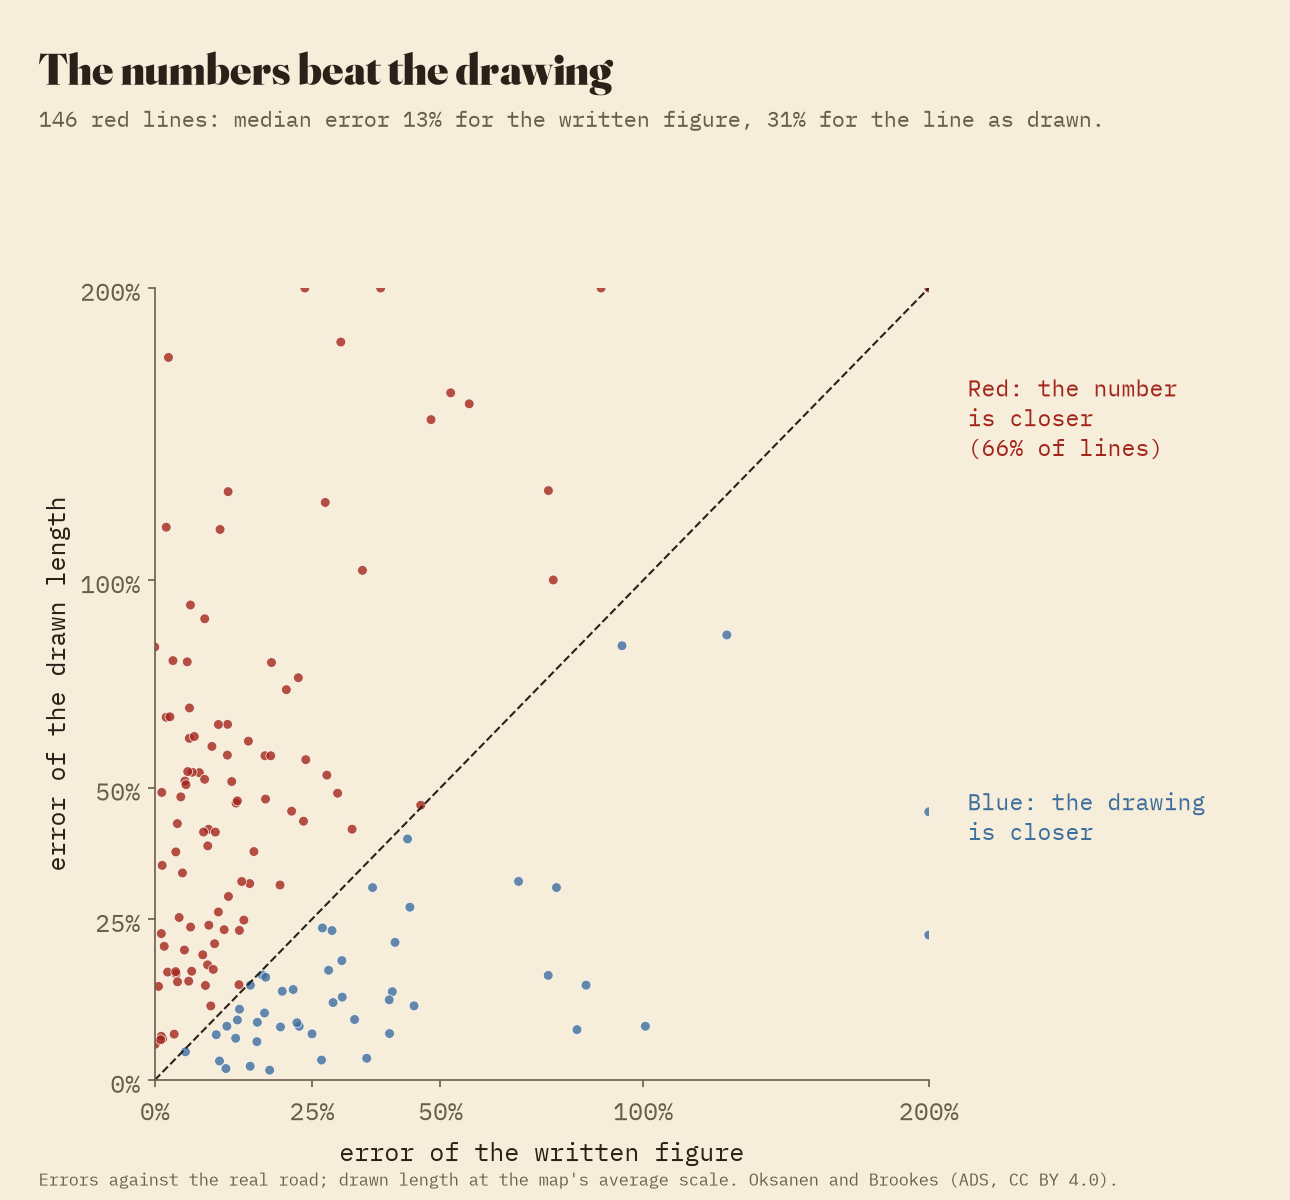
\includegraphics[width=.75\textwidth]{f_drawn.png}
\caption{Absolute error of the written figure (at the median rate) against absolute error of the drawn length, per red line.}\label{fig:drawn}\end{figure}

\subsection{Journeys}
The red lines form 4 connected groups; the largest joins 154 way stations. Summing written figures along the shortest routes from London gives York at 202 miles (420 km against 424 km of road), Bristol at 202 against 203, Carlisle 485 against 493, St David's 445 against 432 and Exeter 343 against 292, the largest discrepancy (Figure~\ref{fig:journeys}).

\begin{figure}[tbp]\centering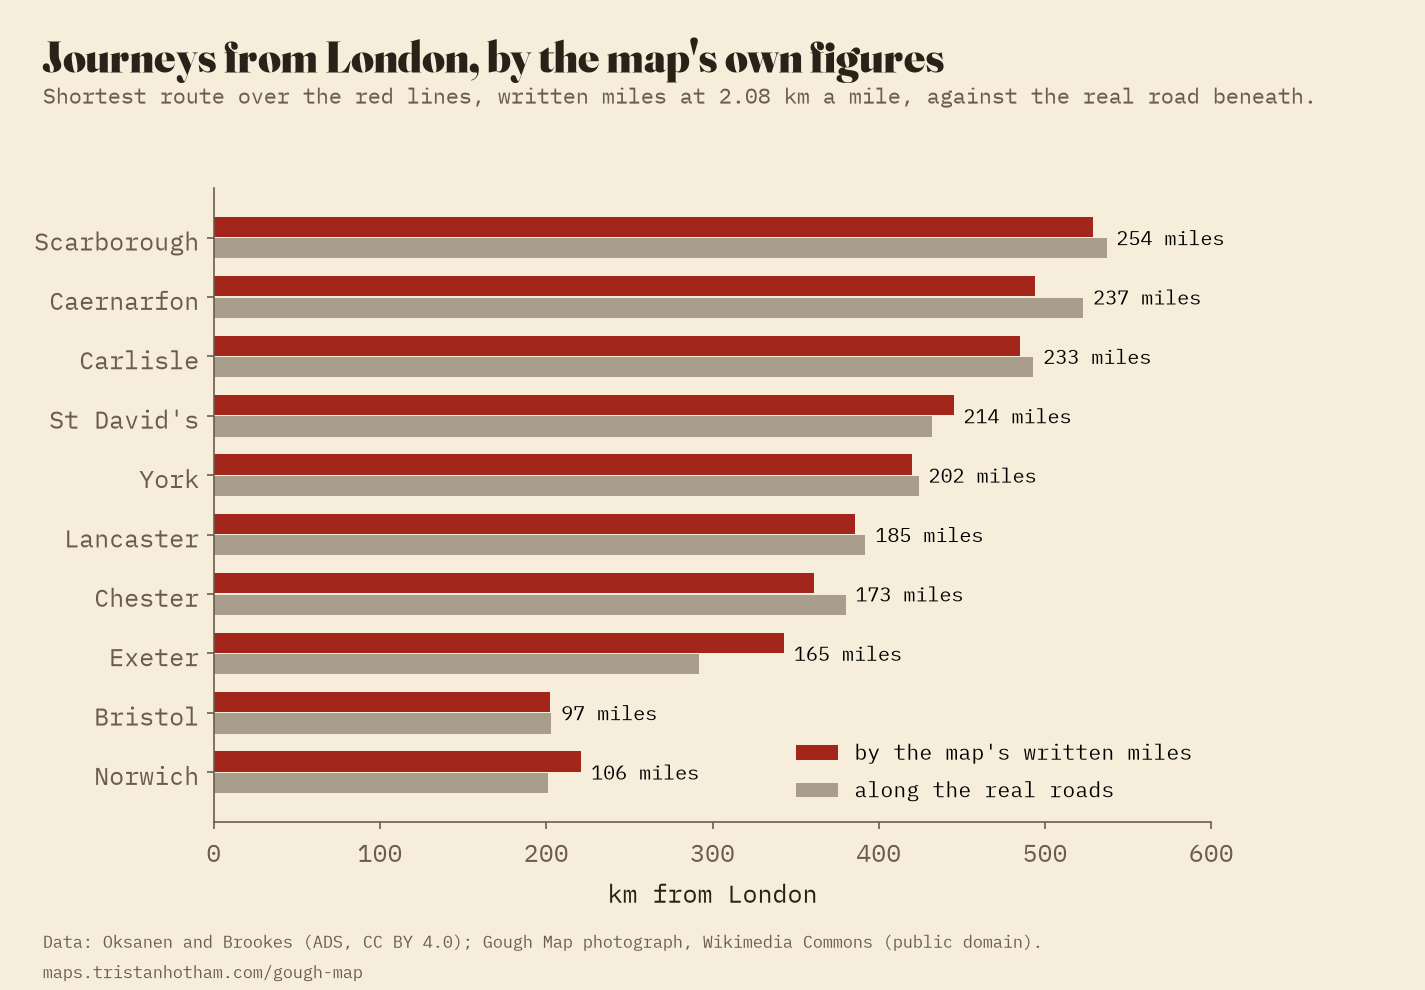
\includegraphics[width=.85\textwidth]{f_journeys.png}
\caption{Journeys from London: written figures summed along the shortest route over the red lines and converted at the median rate, against the road length along the same lines.}\label{fig:journeys}\end{figure}

\subsection{Roads by period}
The red lines use 436 route segments, 4,505 km. By period code, 35.4\% is Roman road, 13.1\% has evidence before 1086, 6.7\% dated medieval evidence, 9.1\% other medieval evidence and 32.7\% is known only from the early modern road books (Figure~\ref{fig:roads}). 71 red lines (38\%) run mostly on Roman road. The rate per written mile is 2.10 km on mainly Roman lines and 2.10 km on lines known only from the road books, with 71\% and 68\% within 25\%.

\begin{figure}[tbp]\centering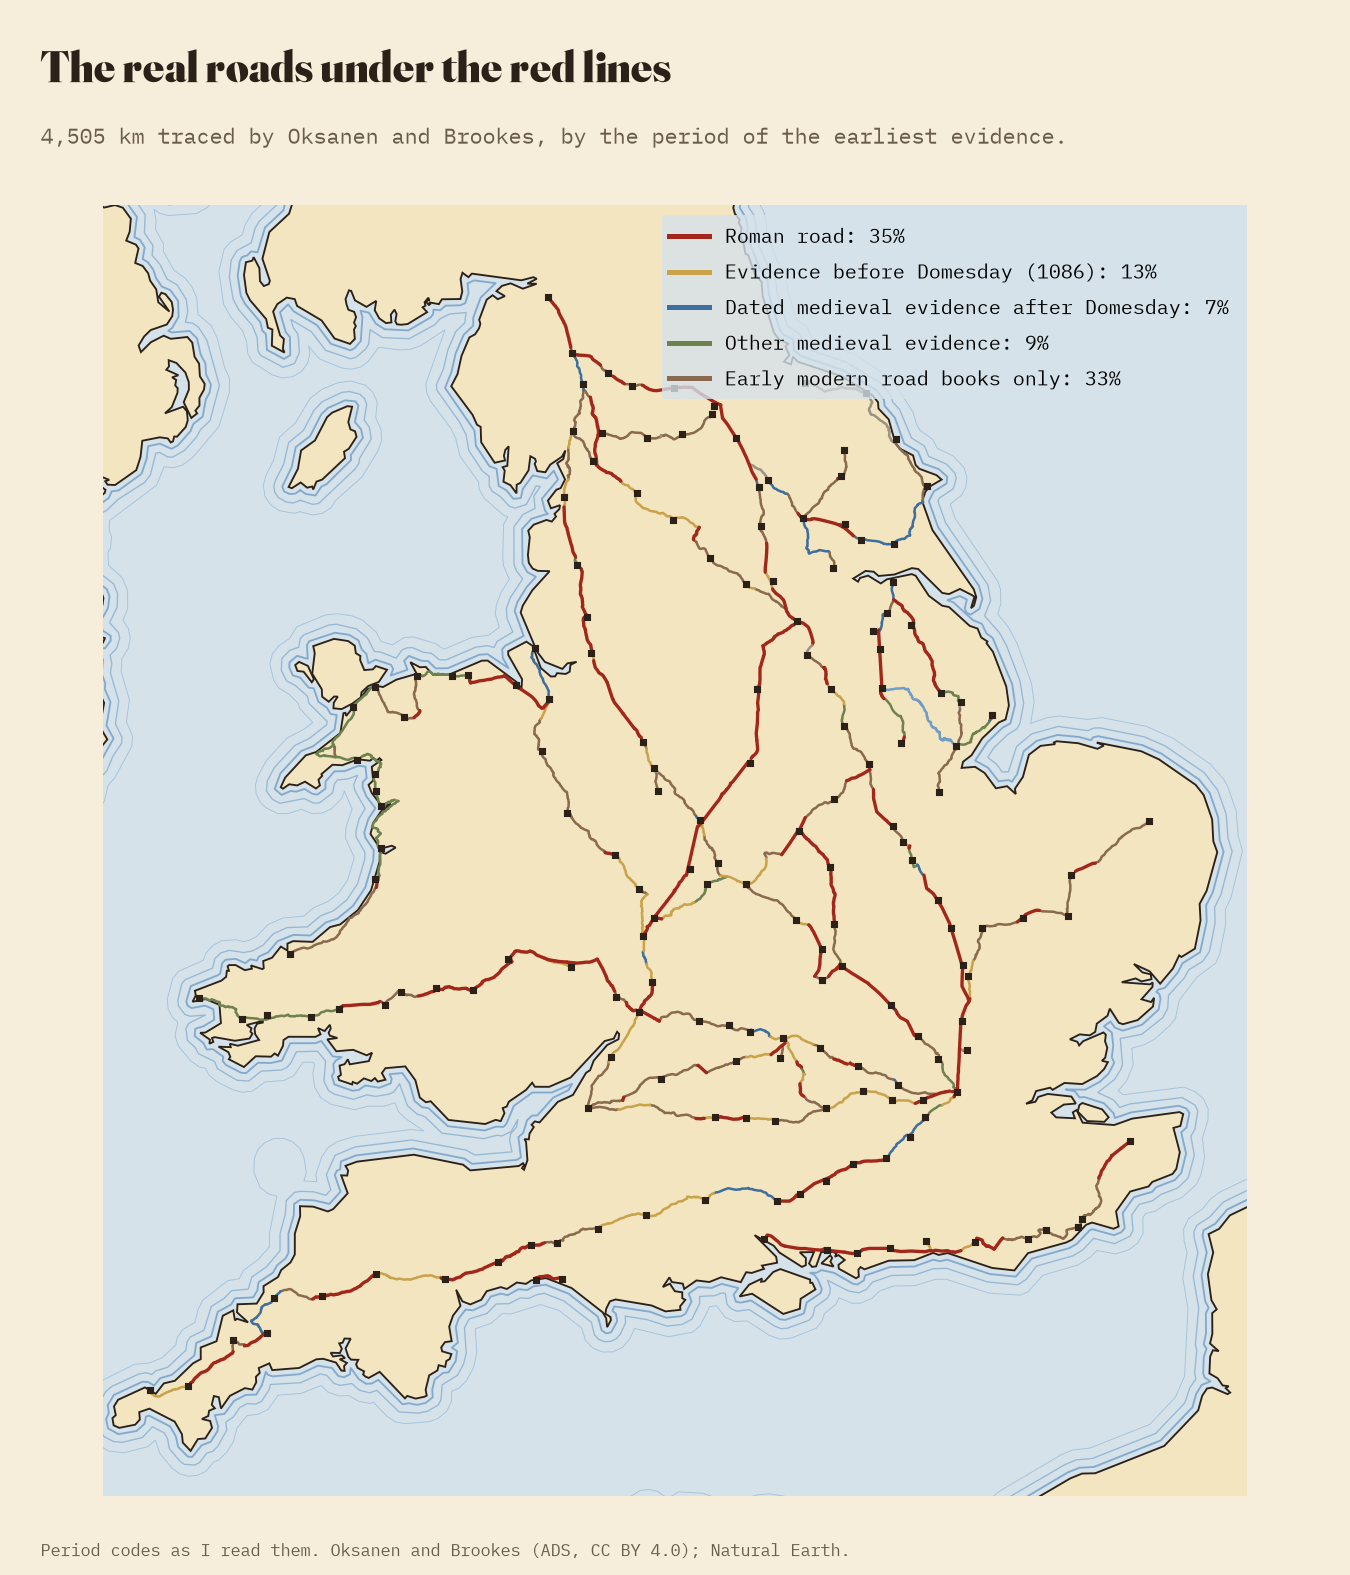
\includegraphics[width=.8\textwidth]{f_roads.png}
\caption{The route segments under the red lines by period code (my reading of the codes), with the way stations.}\label{fig:roads}\end{figure}

\section{Limitations}
The positions on the map are mine, read by eye; 68 are uncertain and 22 are missing, and they favour legible places. Leaving the uncertain ones out moves the rotation by under two degrees and changes no conclusion, but individual misplacements, especially in Wales and the far north of England, should be read with that in mind. The road distances depend on Oksanen and Brookes' identification of the routes, which is itself an argument, and on my reading of the period codes. The similarity and affine fits summarise a map that was never drawn to one projection; the thin-plate spline is only a visual aid. The Scottish control points are few, and some are guesses. The statute mile is used only as a yardstick: the map's mile was a customary unit.

\section{Conclusion}
The Gough Map places the towns of England within a couple of tens of kilometres of where an accurate map at its scale would, and its errors are regional: Wales enlarged and spread, the north slightly shrunk, Scotland squeezed. Its written distances are more reliable than its drawing: in a medieval mile of about 2.08 km of road, most are within a quarter of the truth, and over long journeys the errors cancel. Whoever compiled the red lines worked from distances along roads, many of them Roman, many first recorded centuries later.

\section*{Data and code availability}
Data, code, the interactive page and the positions on the map are at \url{https://github.com/Tristan-Hotham/gough-map} and \url{https://maps.tristanhotham.com/gough-map/}, under the MIT licence (code) and CC BY 4.0 (text, figures and derived data). The road database is CC BY 4.0 \citep{ads}; the photograph is public domain.

\section*{AI statement}
I wrote the text, with drafting and editing assistance from Claude (Anthropic), which also helped prepare the analysis code. I reviewed and checked all text and results.

\begin{thebibliography}{9}
\bibitem[Bookstein(1989)]{bookstein} Bookstein, F. L. (1989) Principal warps: thin-plate splines and the decomposition of deformations. \emph{IEEE Transactions on Pattern Analysis and Machine Intelligence} 11(6), 567-585.
\bibitem[Delano-Smith et~al.(2017)]{delano} Delano-Smith, C. et al. (2017) New light on the medieval Gough Map of Britain. \emph{Imago Mundi} 69(1), 1-36.
\bibitem[Lilley et~al.(2009)]{lilley} Lilley, K. D., Lloyd, C. D. and Campbell, B. M. S. (2009) Mapping the realm: a new look at the Gough map of Britain (c. 1360). \emph{Imago Mundi} 61(1), 1-28.
\bibitem[Margary(1973)]{margary} Margary, I. D. (1973) \emph{Roman Roads in Britain}. 3rd edn. London: John Baker.
\bibitem[Natural Earth(n.d.)]{ne} Natural Earth. Free vector and raster map data at 1:10m, 1:50m and 1:110m scales. Website, \url{https://www.naturalearthdata.com/} (accessed 2026). Public domain.
\bibitem[Ogilby(1675)]{ogilby} Ogilby, J. (1675) \emph{Britannia}. London.
\bibitem[Oksanen and Brookes(2024)]{ads} Oksanen, E. and Brookes, S. (2024) \emph{The Routes and Roads of the Gough Map: GIS Database} [data-set]. York: Archaeology Data Service [distributor]. \url{https://doi.org/10.5284/1124312}.
\bibitem[Parsons(1958)]{parsons} Parsons, E. J. S. (1958) \emph{The Map of Great Britain circa A.D. 1360 known as the Gough Map: An Introduction to the Facsimile}, with ``The roads of the Gough Map'' by Sir Frank Stenton. Oxford: Bodleian Library and Royal Geographical Society.
\bibitem[Tobler(1994)]{tobler} Tobler, W. R. (1994) Bidimensional regression. \emph{Geographical Analysis} 26(3), 187-212.
\end{thebibliography}

\clearpage
{\footnotesize\setlength{\tabcolsep}{4pt}\begin{longtable}{p{5.4cm}p{4.2cm}rrlr}\caption{The 163 places located on the photograph of the Gough Map (12,224 by 6,021 pixels; x to the right, y down), with confidence and misplacement (km) at the overall similarity, by region and name.}\label{tab:located}\\\toprule Place & County & x & y & Read & km\\\midrule\endfirsthead\toprule Place & County & x & y & Read & km\\\midrule\endhead
Barton-upon-Humber & Lincolnshire & 6,600 & 2,320 & med & 14\\
Boston & Lincolnshire & 7,230 & 1,925 & med & 17\\
Bury St Edmunds & Suffolk & 7,860 & 1,230 & high & 26\\
Caistor & Lincolnshire & 6,770 & 2,230 & med & 16\\
Cambridge & Cambridgeshire & 8,060 & 1,595 & high & 16\\
Caxton & Cambridgeshire & 8,155 & 1,800 & high & 7\\
Glanford Brigg & Lincolnshire & 6,720 & 2,390 & med & 20\\
Grantham & Lincolnshire & 7,460 & 2,375 & med & 15\\
Horncastle & Lincolnshire & 7,030 & 2,120 & med & 23\\
Huntingdon & Huntingdonshire & 7,980 & 1,855 & high & 11\\
Lincoln & Lincolnshire & 7,165 & 2,410 & med & 22\\
Newmarket & Cambridgeshire & 7,880 & 1,460 & high & 27\\
Norwich & Norfolk & 7,360 & 950 & high & 30\\
Ogerston & Huntingdonshire & 7,970 & 2,020 & med & 6\\
Old Bolingbroke & Lincolnshire & 7,110 & 2,030 & low & 22\\
Sleaford & Lincolnshire & 7,254 & 2,235 & low & 20\\
Spalding & Lincolnshire & 7,550 & 1,905 & low & 5\\
Spital-in-the-Street & Lincolnshire & 7,020 & 2,410 & med & 20\\
Stamford & Lincolnshire & 7,720 & 2,200 & med & 12\\
Thetford & Norfolk & 7,700 & 1,180 & med & 24\\
Wainfleet & Lincolnshire & 7,050 & 1,900 & med & 28\\
Birmingham & Warwickshire & 7,720 & 2,990 & low & 33\\
Blyth & Nottinghamshire & 6,830 & 2,710 & low & 24\\
Bridgnorth & Shropshire & 8,000 & 3,610 & low & 24\\
Chester & Cheshire & 7,280 & 3,720 & high & 3\\
Chesterfield & Derbyshire & 6,890 & 2,785 & low & 30\\
Coleshill & Warwickshire & 7,830 & 2,765 & low & 22\\
Coventry & Warwickshire & 8,020 & 2,700 & med & 9\\
Daventry & Northamptonshire & 8,170 & 2,490 & med & 7\\
Derby & Derbyshire & 7,090 & 2,746 & low & 44\\
Droitwich & Worcestershire & 7,960 & 3,080 & low & 34\\
Hereford & Herefordshire & 8,640 & 3,570 & high & 11\\
Kidderminster & Worcestershire & 8,070 & 3,390 & low & 17\\
Leicester & Leicestershire & 7,515 & 2,672 & med & 34\\
Lichfield & Staffordshire & 7,460 & 2,920 & low & 36\\
Market Harborough & Leicestershire & 7,800 & 2,455 & low & 20\\
Melton Mowbray & Leicestershire & 7,362 & 2,665 & low & 42\\
Newark-on-Trent & Nottinghamshire & 7,335 & 2,520 & high & 16\\
Northampton & Northamptonshire & 8,150 & 2,310 & high & 9\\
Overton & Cheshire & 7,560 & 3,810 & med & 6\\
Shrewsbury & Shropshire & 7,880 & 3,850 & med & 25\\
Solihull & Warwickshire & 7,870 & 2,870 & low & 24\\
Towcester & Northamptonshire & 8,330 & 2,370 & low & 3\\
Tuxford & Nottinghamshire & 7,130 & 2,630 & low & 20\\
Wansford & Northamptonshire & 7,820 & 2,110 & high & 7\\
Worcester & Worcestershire & 8,460 & 3,200 & high & 9\\
Appleby-in-Westmorland & Westmorland & 5,870 & 3,520 & low & 12\\
Beverley & Yorkshire, East Riding & 6,430 & 2,290 & med & 10\\
Boroughbridge & Yorkshire, West Riding & 6,230 & 3,060 & low & 22\\
Bowes & Yorkshire, North Riding & 5,895 & 3,190 & low & 12\\
Bridlington & Yorkshire, East Riding & 6,450 & 2,130 & low & 29\\
Brough & Westmorland & 5,770 & 3,470 & low & 5\\
Castle Bolton & Yorkshire, North Riding & 6,230 & 3,295 & low & 22\\
Doncaster & Yorkshire, West Riding & 6,720 & 2,865 & low & 29\\
Gilling & Yorkshire, North Riding & 6,030 & 3,115 & low & 16\\
Guisborough & Yorkshire, North Riding & 5,720 & 2,560 & med & 11\\
Hadrian's Wall, east end (Wallsend) & Northumberland & 5,060 & 2,850 & med & 27\\
Hadrian's Wall, west end (Bowness-on-Solway) & Cumberland & 5,320 & 3,740 & med & 34\\
Helperby & Yorkshire, North Riding & 6,230 & 2,880 & low & 8\\
Kendal & Westmorland & 6,080 & 3,680 & low & 6\\
Kirkby Lonsdale & Westmorland & 6,210 & 3,620 & low & 3\\
Lancaster & Lancashire & 6,380 & 3,700 & med & 5\\
Leeming Bar & Yorkshire, North Riding & 6,040 & 2,995 & low & 4\\
Liverpool & Lancashire & 7,050 & 3,820 & low & 2\\
Malton & Yorkshire, North Riding & 6,430 & 2,540 & low & 28\\
Penrith & Cumberland & 5,650 & 3,640 & low & 13\\
Pickering & Yorkshire, North Riding & 6,280 & 2,530 & low & 26\\
Pontefract & Yorkshire, West Riding & 6,560 & 2,895 & low & 19\\
Preston & Yorkshire & 6,690 & 3,680 & med & 3\\
Richmond & Yorkshire, North Riding & 6,100 & 3,180 & low & 20\\
Scarborough & Yorkshire, North Riding & 6,190 & 2,420 & low & 30\\
Settle & Yorkshire, West Riding & 6,230 & 3,440 & low & 9\\
Shap & Westmorland & 5,880 & 3,640 & low & 8\\
Skipton & Yorkshire, West Riding & 6,210 & 3,330 & low & 24\\
Wakefield & Yorkshire, West Riding & 6,505 & 3,030 & low & 25\\
Warrington & Lancashire & 7,060 & 3,550 & low & 2\\
Whitby & Yorkshire, North Riding & 5,940 & 2,480 & med & 21\\
Wigan & Lancashire & 6,880 & 3,580 & low & 3\\
York & Yorkshire, West Riding & 6,420 & 2,780 & high & 16\\
Bass Rock & Scotland & 3,850 & 3,410 & med & 49\\
Isle of May & Scotland & 3,550 & 3,080 & med & 83\\
Orkney (Mainland) & Scotland & 1,900 & 2,050 & low & 246\\
Perth & Scotland & 4,140 & 3,720 & low & 68\\
Abingdon & Berkshire & 8,910 & 2,680 & low & 16\\
Alton & Hampshire & 9,500 & 2,070 & high & 21\\
Arundel & Sussex & 9,704 & 1,765 & low & 19\\
Barkway & Hertfordshire & 8,290 & 1,645 & high & 16\\
Battle & Sussex & 9,550 & 1,095 & low & 14\\
Boreham Street & Sussex & 9,605 & 1,275 & med & 5\\
Bramber & Sussex & 9,686 & 1,622 & low & 16\\
Brentford & Middlesex & 8,800 & 1,835 & med & 23\\
Burford & Oxfordshire & 8,830 & 2,810 & low & 8\\
Canterbury & Kent & 9,075 & 665 & high & 22\\
Chichester & Sussex & 9,715 & 1,815 & high & 29\\
Colnbrook & Buckinghamshire & 9,020 & 2,020 & med & 4\\
Dunstable & Bedfordshire & 8,560 & 2,020 & high & 4\\
Faringdon & Berkshire & 9,020 & 2,720 & med & 11\\
Farnham & Surrey & 9,420 & 2,010 & high & 16\\
Guildford & Surrey & 9,300 & 1,800 & low & 20\\
Havant & Hampshire & 9,740 & 1,990 & med & 25\\
High Barnet & Hertfordshire & 8,790 & 1,730 & med & 8\\
Hungerford & Berkshire & 9,380 & 2,570 & low & 23\\
Kingston & Surrey & 9,020 & 1,845 & low & 9\\
Lewes & Sussex & 9,672 & 1,550 & med & 1\\
London & Middlesex & 8,840 & 1,610 & high & 16\\
Maidenhead & Berkshire & 9,045 & 2,150 & med & 4\\
New Alresford & Hampshire & 9,545 & 2,120 & med & 27\\
Newbury & Berkshire & 9,300 & 2,550 & med & 12\\
Oxford & Oxfordshire & 8,790 & 2,490 & high & 3\\
Reading & Berkshire & 9,060 & 2,440 & med & 15\\
Royston & Hertfordshire & 8,320 & 1,750 & high & 8\\
Rye & Sussex & 9,375 & 860 & med & 26\\
Southampton & Hampshire & 9,780 & 2,235 & high & 31\\
St Albans & Hertfordshire & 8,665 & 1,855 & high & 8\\
Stony Stratford & Buckinghamshire & 8,470 & 2,270 & med & 4\\
Tetsworth & Oxfordshire & 8,810 & 2,260 & med & 9\\
Uxbridge & Middlesex & 8,910 & 2,040 & med & 9\\
Waltham Holy Cross & Essex & 8,705 & 1,665 & high & 8\\
Ware & Hertfordshire & 8,510 & 1,715 & high & 14\\
Winchelsea & Sussex & 9,555 & 1,010 & med & 7\\
Winchester & Hampshire & 9,590 & 2,320 & high & 18\\
Witney & Oxfordshire & 8,800 & 2,700 & low & 3\\
Bridport & Dorset & 10,120 & 3,250 & low & 25\\
Bristol & Gloucestershire & 9,230 & 3,190 & high & 22\\
Chard & Somerset & 9,940 & 3,515 & low & 14\\
Crewkerne & Somerset & 9,910 & 3,285 & low & 23\\
Exeter & Devonshire & 10,140 & 3,860 & high & 18\\
Gloucester & Gloucestershire & 8,890 & 3,105 & high & 19\\
Honiton & Devonshire & 10,060 & 3,690 & low & 14\\
Lyme Regis & Dorset & 10,170 & 3,450 & low & 21\\
Malmesbury & Wiltshire & 9,100 & 2,950 & med & 15\\
Marlborough & Wiltshire & 9,300 & 2,730 & med & 14\\
Newent & Gloucestershire & 8,740 & 3,320 & med & 8\\
Newport & Gloucestershire & 9,100 & 3,205 & med & 19\\
Northleach & Gloucestershire & 8,810 & 2,950 & low & 7\\
Okehampton & Devonshire & 10,220 & 4,260 & med & 19\\
Salisbury & Wiltshire & 9,690 & 2,600 & high & 26\\
Shaftesbury & Dorset & 9,760 & 2,930 & med & 19\\
Sherborne & Dorset & 9,810 & 3,225 & med & 11\\
Aberdovey & Merionethshire & 8,100 & 5,110 & med & 66\\
Abergele & Denbighshire & 7,180 & 4,280 & low & 10\\
Aberystwyth & Cardiganshire & 8,520 & 5,100 & med & 70\\
Bangor & Carnarvonshire & 7,080 & 4,600 & high & 24\\
Barmouth & Merionethshire & 7,910 & 5,100 & low & 63\\
Brecon & Brecknockshire & 8,880 & 4,030 & med & 20\\
Caernarfon & Carnarvonshire & 7,090 & 4,830 & med & 38\\
Capel Curig & Carnarvonshire & 7,210 & 4,510 & med & 26\\
Cardigan & Cardiganshire & 8,900 & 4,940 & med & 33\\
Carmarthen & Carmarthenshire & 9,170 & 4,640 & med & 35\\
Clyro & Radnorshire & 8,740 & 3,830 & med & 22\\
Conwy & Carnarvonshire & 7,220 & 4,410 & med & 5\\
Criccieth & Carnarvonshire & 7,490 & 5,095 & med & 52\\
Flint & Flintshire & 7,330 & 3,960 & low & 10\\
Harlech & Merionethshire & 7,720 & 5,130 & low & 62\\
Haverfordwest & Pembrokeshire & 9,330 & 5,030 & med & 43\\
Llandeilo & Carmarthenshire & 8,940 & 4,510 & low & 20\\
Llanenddwyn & Merionethshire & 7,800 & 5,110 & low & 61\\
Llangadog & Carmarthenshire & 8,950 & 4,400 & low & 25\\
Llawhaden & Pembrokeshire & 9,230 & 4,880 & low & 36\\
Llywel & Brecknockshire & 8,945 & 4,240 & low & 27\\
Rhuddlan & Flintshire & 7,290 & 4,090 & low & 8\\
St Clears & Carmarthenshire & 9,200 & 4,730 & low & 33\\
St David's & Pembrokeshire & 9,190 & 5,230 & high & 37\\
\bottomrule\end{longtable}}
\end{document}
